\section{Complex Behavior through custom Action Sampling Distributions}
\begin{figure}
	\centering
	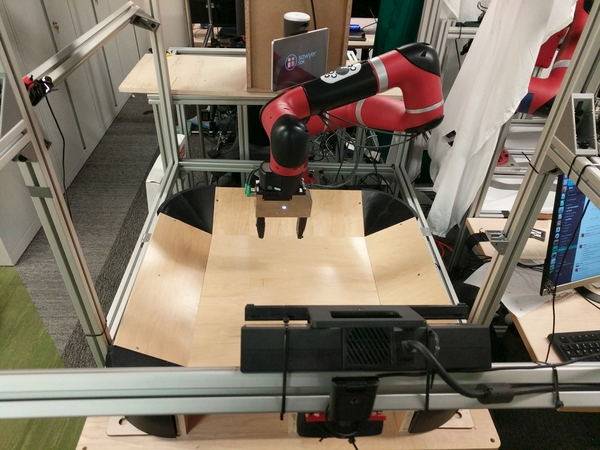
\includegraphics[width=1.0\linewidth]{images_general/robot_setup.jpg}
	\caption{\small{Robot setup, with 2 standard web-cams arranged at different viewing angles. \todo{highlight cameras!}}
		\label{fig:robot_setup}
	}
\end{figure}
\label{sec:system}
When collecting data by sampling from simple distributions, such as a multivariate Gaussian, the skills that emerged were found to be generally restricted to pushing and dragging objects. This is because with simple distributions, it is very unlikely to visit states like picking up and placing of objects or folding cloth. Not only would the model be imprecise for these kinds of states, but also during planning it would be unlikely to \emph{find} action sequences that grasp an object or fold a piece of cloth. 
We therefore explore how the sampling distribution used both in data collection and sampling-based planning can be changed to visit these, otherwise unlikely, states more frequently, allowing more complex behavior to emerge. 

\textbf{Learning complex Pick and Place Behavior:}

We first discuss picking and placing of objects. To allow picking up and placing of objects to occur more frequently, we incorporate a simple ``reflex'' during data collection, where the gripper automatically closes, when the height of the wrist above the table is lower than a small threshold. This reflex is inspired by the palmar reflex observed in infants~\cite{grasping_fetal}. With this primitive, about 20\% of training trajectories included some sort of grasp on an object. It is worth noting that, other than this reflex, no grasping-specific engineering was applied to the policy allowing a joint pushing and grasping policy to emerge, see figure \ref{fig:push_grasp}. In our experiments, we evaluate our method using data obtained both with and without the grasping reflex, evaluating both purely non-prehensile and combined prehensile and non-prehensile manipulation.

\textbf{Learning Deformable Object Manipulation}
In order to collect meaningful interaction data for learning folding of deformable objects such as towels and cloths, we adapted the sampling distribution to increase the likelihood of encountering ``cloth-folding-states`` in the data. When using actions sampled from a simple distribution or the distribution used for grasping collection, cloths would become tangled up and we would see a lot of ``sweeping motions``. To improve the efficiency of encountering ``cloth folds``, we use the same action primitive used both for grasping primitive, but additionally we reduce lateral motion of the end-effector when the gripper is close to the table, thus reducing the undesired ``sweeping motions``.
%%SL.10.15: Have transition here and explain what this section is about. Currently, it seems like a bunch of disjointed miscallaneous stuff that didn't fit in anywhere else. This is not good. Maybe you can call this system design and describe the robot setup here first (both single view and multi-view), then details about data collection -- how actions are selected etc. (which can be merged with 7.2). Figures would help to illustrate the robot setup. 7.3 probably doesn't belong here at all, but belongs in experiments

\section{Multi-View Visual MPC}
The visual MPC algorithm as described so far is only able to solve manipulation tasks specified in 2D, like rearranging objects on the table, however a task such as lifting an object to a particular position in 3D cannot be fully specified with a single view, since it would be ambiguous. 

We use a combination of multiple views, taken with multiple cameras arranged appropriately, to jointly define a 3D task. Figure \ref{fig:robot_setup} shows the robot setup, including 2 standard webcams observing the workspace from different angles. The registration method described in the previous section is used separately per view to allow for dynamic retrying and solving temporally extended tasks. The planning costs from each view are combined using weighted averaging where the weights are provided by the registration network (see equation \ref{eqn:cost_avg}).  \todo{Figure XX shows an example lifting task, which specified in two views.}

The classifier-based cost is also used in the multiview-setup, an example trajectory of cloth folding is shown \todo{in figure}. 





